\documentclass[preprint,11pt]{aastex}

\begin{document}

\title{The Panchromatic Hubble Andromeda Treasury. XXX. Calibrating ultraviolet
    and infrared star formation tracers as a function of environment.
}

\author{Jacob E. Simones}

\and

\author{
    Julianne J. Dalcanton,
    Andrew E. Dolphin,
    Alexia R. Lewis,
    Evan D. Skillman,
    Daniel R. Weisz,
    Benjamin F. Williams
}





\section{Summary}

The proposed project is in many ways similar to the pilot study
\citep{Simones14}: measure SFRs for a set of regions based on integrated fluxes
of a particular tracer and compare with the mean SFRs from the derived SFHs.
The main difference is that we will have full control over the sample design,
whereas the pilot sample contained only UV-bright regions and was limited in
the range of physical sizes.

The overall concept of the project is to compare SFR maps from integrated
tracer emission with a SFR map obtained from PHAT SFHs. We will consider at
minimum FUV flux as a SF tracer, though if possible, I would like to include
FUV+$24\,\mathrm{\mu m}$ as well. Other currently available data include GALEX
NUV, and Spitzer/MIPS 70 and $160\,\mathrm{\mu m}$. Comparisons can be made on
a pixel-by-pixel basis in the maps, and also on the basis of larger regions,
e.g., representing different slices in galactic radius and surface brightness.

The purpose of this document is to clearly define the project and establish the
main science questions at the beginning. This way, everyone involved will be on
the same page and we will be able to move forward as efficiently as possible.





\section{Data}

\subsection{SFR map}

Alexia has calculated SFHs for all bricks except 1 and 3 in the bulge (Figure
\ref{fig:map}), with each brick divided into 450 rectangular subregions, or
``pixels'' (to distinguish from the term ``regions'', which will refer to
larger areas made from groups of pixels). There are 9450 pixels total, each one
approximately $25\arcsec$ per side. I have the following data in hand:
\begin{itemize}
\item Coordinates of the region corners in RA and dec
\item F475W and F814W photometry
\item Best-fit SFH for each pixel:

    \begin{itemize}
    \item $A_{\mathrm{V},f}$ and $dA_\mathrm{V}$ extinction parameters
    \item Model CMD data
    \item SFR and $\mathrm{[M/H]}$ vs. $t$
    \end{itemize}

\item Uncertainties:

    \begin{itemize}
    \item Random uncertainties from the HMC routine. All pixels.
    \item Systematics due to isochrone uncertainties. Select pixels only.
        \emph{In progress}
    \item Systematics due to uncertainties in the
        $A_{\mathrm{V},f},dA_\mathrm{V}$ parameters. All pixels? \emph{In
        progress}.
    \end{itemize}

\end{itemize}

For each SFR tracer of interest, I will average the SFHs in the pixels over the
relevant timescale, $\Delta t$ (e.g., the last $100\,\mathrm{Myr}$ for the FUV
tracer) to obtain maps of the mean SFRs, $\langle \mathrm{SFR}\rangle_{\Delta
t}$. The uncertainties in $\langle \mathrm{SFR}\rangle_{\Delta t}$ will be
evaluated as described in \citet{Simones14}.

An extinction map is required for UV dust corrections. Ideally, an extinction
map would be derived from just the best-fit $A_{\mathrm{V},f}$ and
$dA_\mathrm{V}$ extinction parameters in each pixel. Doing so ensures
self-consistency in the analysis and keeps the list of assumptions to a minimum
(those already made by MATCH). The simplest approach is to calculate the mean
total extinction, $A_{\mathrm{V},f} + dA_\mathrm{V}/2$. The more accurate
approach is that of Ben Johnson, who modeled the intrinsic and reddened
(according to the same $A_{\mathrm{V},f},dA_\mathrm{V}$ extinction model) FUV
magnitudes in \citet{Simones14}: 1) the modeled intrinsic spectrum is split up
into several parts, emulating multiple lines of sight; 2) a value of
$A_\mathrm{V}$ is drawn from a uniform distribution between $A_{\mathrm{V},f}$
and $A_{\mathrm{V},f} + dA_\mathrm{V}$ for each sight line; 3) the reddened
spectra along the sight lines are added up to get the total reddened spectrum,
which is converted to an FUV magnitude; 4) the difference between the intrinsic
and reddened FUV magnitudes is the total FUV extinction. The challenge with
this approach will be finding a method for estimating the total FUV extinction
in a way that does not depend on the source spectrum (this is in progress).

There are a couple of issues that will need to be resolved before a final
$\langle \mathrm{SFR}\rangle_{\Delta t}$ map can be constructed:
\begin{itemize}
\item Some of the pixels overlap each other. Should their $\langle
    \mathrm{SFR}\rangle_{\Delta t}$ values and uncertainties somehow be
    combined? The easiest approach would be to not combine overlapping data and
    choose one pixel over the other.
\item The pixels are not on a uniform grid, resulting in overlapping pixels
    between bricks and pixels in one location of the map being rotated with
    respect to other locations. Should the SFR map be resampled onto a uniform
    grid? One way to do this is to choose a new pixel size (comparable to the
    original pixel size or larger, as the UV and $24\,\mathrm{\mu m}$ data have
    much smaller pixel scales) and draw a grid inside the boundaries of the
    PHAT survey. I would then add and subtract the SFHs as needed to obtain the
    SFH in each new pixel, from which $\langle \mathrm{SFR}\rangle_{\Delta t}$
    can be calculated.
\end{itemize}

\textbf{Timeline:} Final $\langle \mathrm{SFR}\rangle_{\Delta t}$, uncertainty,
and extinction maps should be obtained by June 1st. This step will require more
new code to be written than any other step in the project (on top of what
already exists from the pilot). It will also require experimentation to find
reasonably-optimal methods for transforming the SFR data (including
uncertainties) into a usable map. I allocate 1 week for constructing a polygon
mesh (or some other representation) of $\langle \mathrm{SFR}\rangle_{\Delta t}$
values, and 1 week to refine the map by dealing with overlap and griding
issues. With the map-making process established, I allocate 1 week to compute
the corresponding uncertainty and extinction maps. Despite my best efforts to
code everything efficiently, computation may become a bottleneck and I should
prepare to secure additional processors (e.g., \texttt{vesuvius.spa.umn.edu},
\texttt{titanus.spa.umn.edu}).


\begin{figure}
\centering
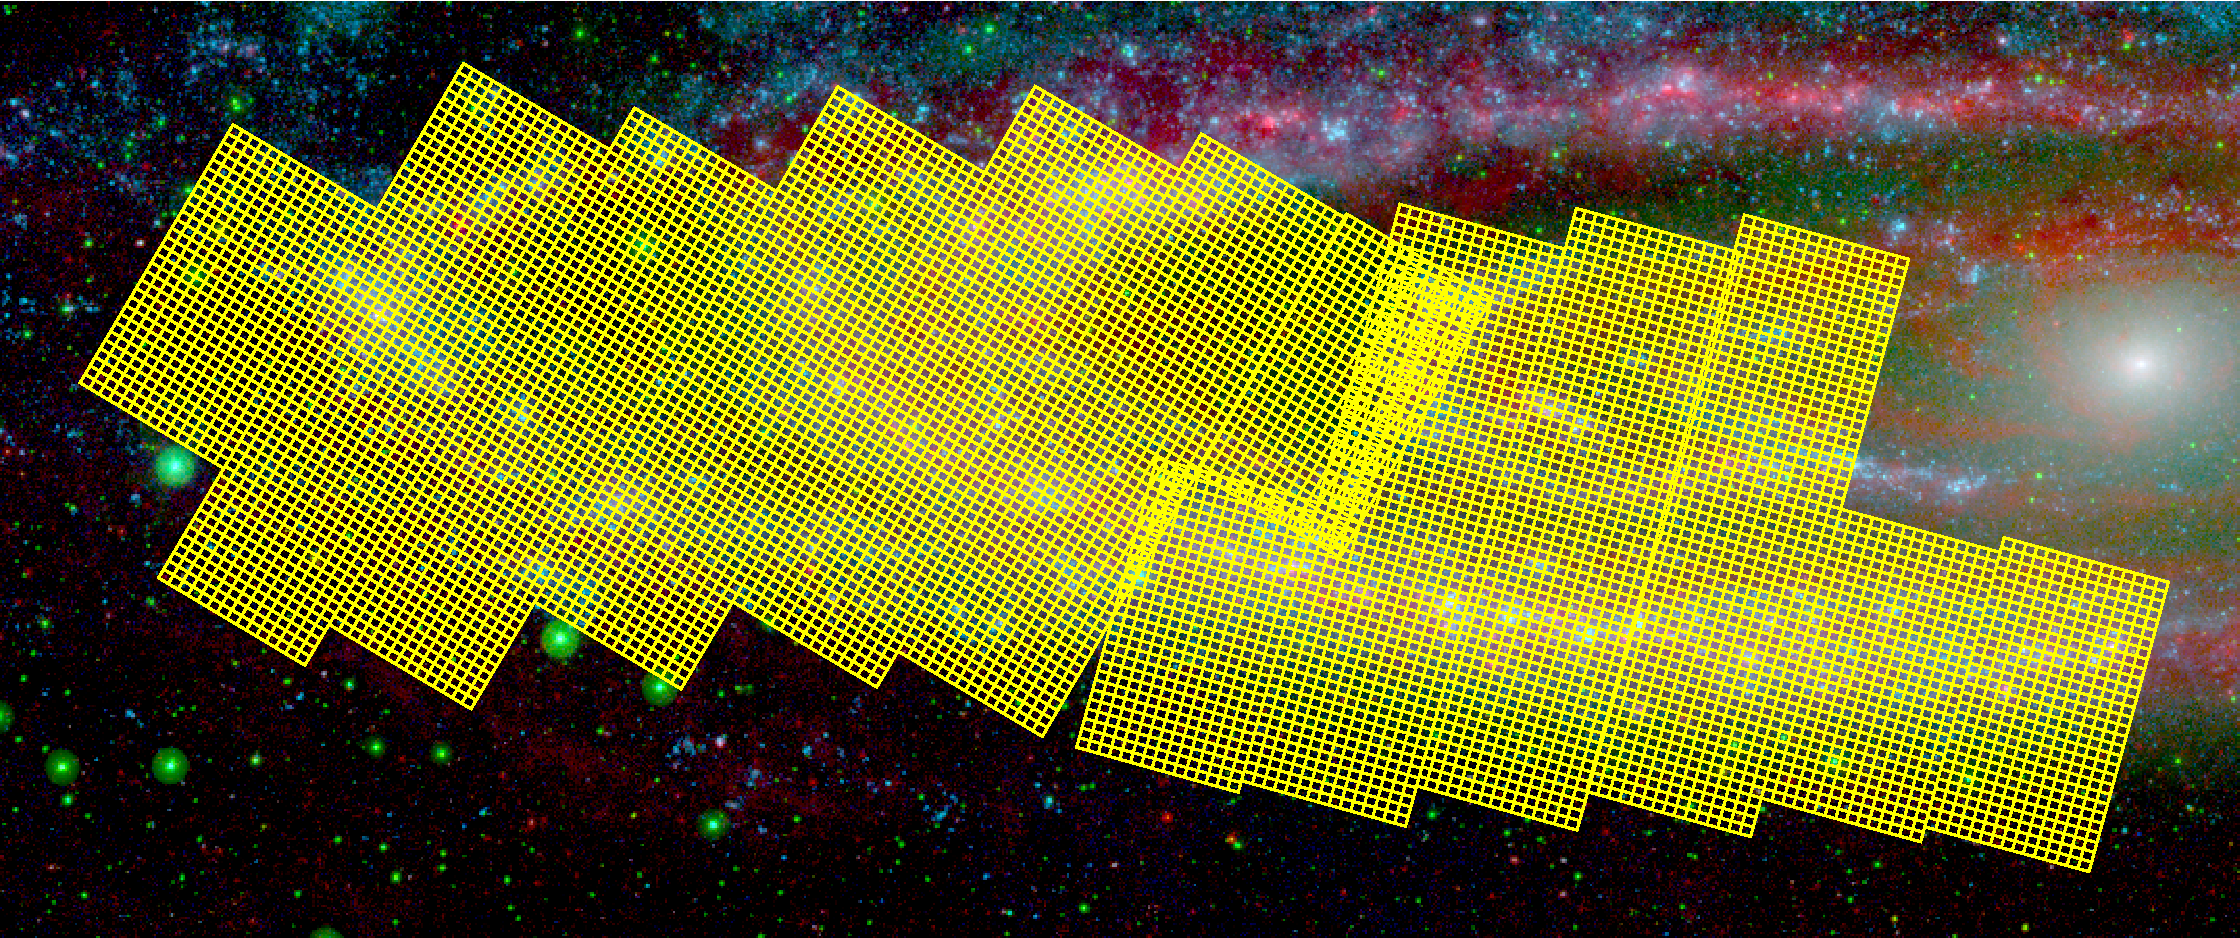
\includegraphics[angle=-90,scale=0.52]{quick_rgb.pdf}
\caption{SFH pixel footprints over an RGB image of M31 (red: Spitzer
    $24\,\mathrm{\mu m}$, green: GALEX NUV, blue: GALEX FUV).
}
\label{fig:map}
\end{figure}



\subsection{GALEX mosaic}

I have made GALEX FUV and NUV mosaics using Montage. The only remaining tasks
are to double-check the WCS alignment with the Spitzer data (if we use it) and
to confirm that flux has been conserved to a satisfactory degree with respect
to the input FUV and NUV images. With a pixel scale of $1.5\arcsec$ (much
smaller than the SFH pixel size), I do not expect this to be an issue.

If anyone knows of science-grade FUV and NUV mosaics that we can use, please
tell me.

\textbf{Timeline:} This should only take a day or two, maybe a couple more if
something goes wrong and I have to remake some mosaics.



\subsection{Spitzer $24\,\mathrm{\mu m}$ mosaic}

Karl Gordon kindly supplied us with Spitzer/MIPS 24, 70, and $160\,\mathrm{\mu
m}$ mosaics of M31. I still need to learn a bit more about how these were
created, but for now I am assuming they are acceptable to use. The pixel scale
of the $24\,\mathrm{\mu m}$ image is approximately $1.2\arcsec$ (smaller than
the documented MIPS pixel scale for the $24\,\mathrm{\mu m}$ channel). As with
GALEX, this is much smaller than the size a SFH pixel.





\section{Tracers}

\citet{Kennicutt12} offer calibrations for FUV, NUV, $24\,\mathrm{\mu m}$,
$70\,\mathrm{\mu m}$, FUV+$24\,\mathrm{\mu m}$, and NUV+$24\,\mathrm{\mu m}$.
It might also be worth considering the FUV and FUV+$24\,\mathrm{\mu m}$
calibrations from \citet{Leroy12}, the FUV calibration from \citet{Salim07}, as
well as calibrations by other authors. At the very least, we will be comparing
the SFH-based SFRs with SFRs from the FUV calibration. The next highest
priority will be FUV+$24\,\mathrm{\mu m}$. Beyond that, the pipeline will be
developed enough that trying out other types of calibrations will be trivial
(assuming the same input GALEX and Spitzer data).





\section{Science}

\textbf{Main questions:}
\begin{itemize}
\item How accurate is a given flux calibration for measuring SFR?
\item How precise is it?
\item Are accuracy and precision affected by environment (e.g., radius and
    surface brightness)?
\item Are there any limitations for this tracer \citep[from][we already know
    that small areas/populations being problematic]{Simones14}?
\end{itemize}

\textbf{Main products:}
\begin{itemize}
\item Measurement of the uncertainties associated with using a particular flux
    calibration.
\item A new calibration for at least FUV, perhaps as a function of environment
    and an overall value.
\end{itemize}

The main questions and products of the paper will guide the sample design. The
two-dimensional approach that was proposed during the Fall 2013 PHAT team
meeting still seems appropriate: divide up the survey area by surface
brightness (proxy for SFR) and radius (proxy for metallicity). A simple version
of this is shown in Figure \ref{fig:regions}. One suggestion that was brough up
at the meeting was to base the regions on structure in the galaxy (e.g., entire
spirals) instead of radial cuts. Exactly how we decide to do this will require
some discussion, though drawing a new set of regions and getting results should
not be too time-consuming, especially doing it one time through.

The most basic set of regions are just the SFH pixels themselves, which are
much larger than the pixels in the UV and $24\,\mathrm{\mu m}$ images. This
would allow us to do a pixel-by-pixel comparison of the flux-based and mean
SFRs. A map of the SFR discrepancies could be very interesting, especially if
there are spatial trends with where the flux calibrations work and where they
don't.

Whatever regions are used, I will have to make sure that their SFHs are all
relatively constant and that high-mass stars are well-represented in the CMDs
to make sure that any observed discrepancies are not due to inconsistencies
with the full-IMF and constant-SFR assumptions. We should also consider
toetallicity effects. For example, what is the radial metallicity gradient in
M31 and what are the final metallicities determined by MATCH?

Most if not all of the functionality required to extract fluxes and SFRs within
arbitrary regions on a map has already been developed during the pilot project.
Getting everything set up should only take a day.

Once all decisions have been made and a basic pipeline is place, it should only
take a couple of days to do test runs and generate plots. The easiest way to
complete a prototype is with a ``$5\times 5$ grid'' in surface brightness and
radius, as shown in Figure \ref{fig:regions}. This is also a good time take a
step back and evaluate the entire pipeline for efficiency, to make sure that it
is scalable to the entire PHAT survey area.

\begin{figure}
\centering
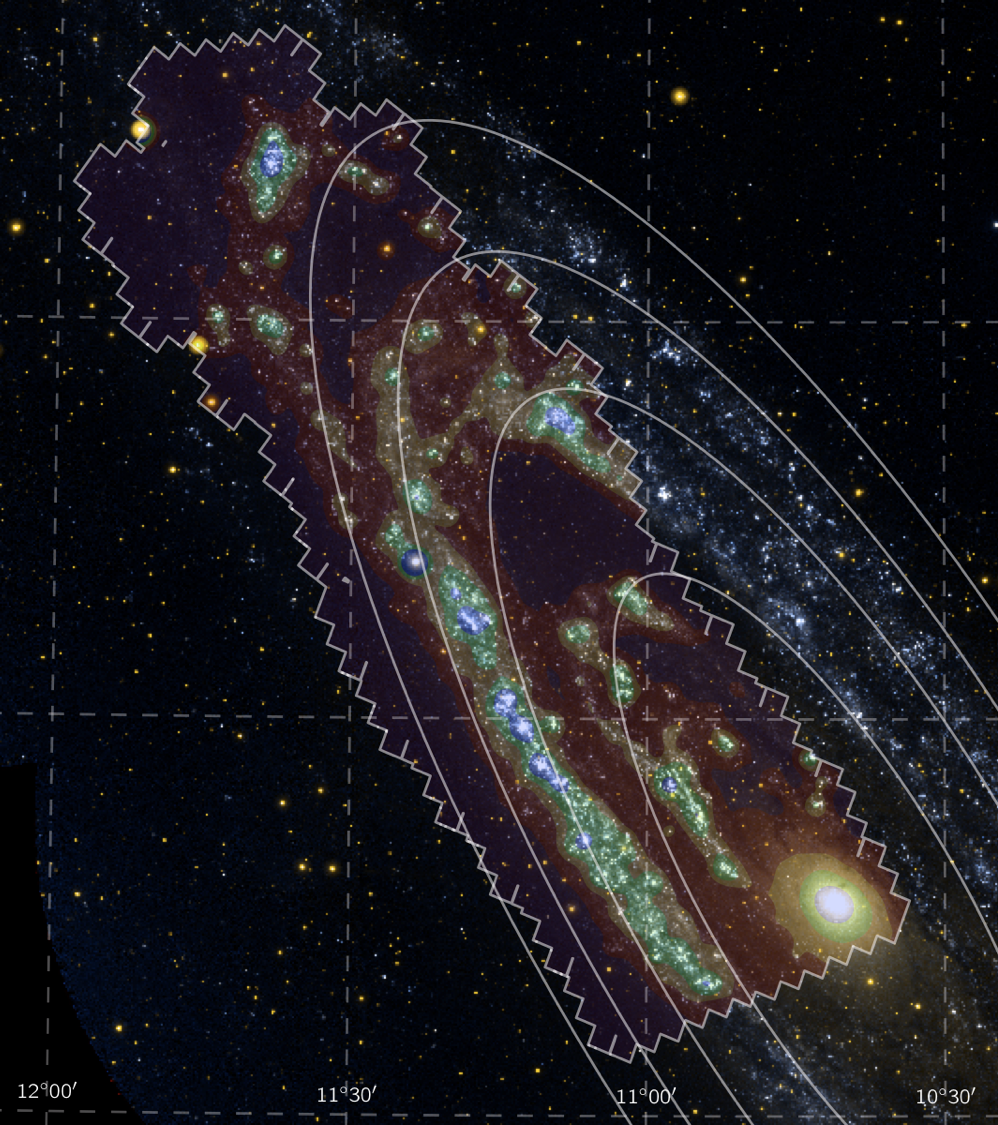
\includegraphics[scale=0.9]{regions.pdf}
\caption{An example region sample defined by 5 sections in radius and 5 levels
    in FUV surface brightness (lowest to highest: purple, red, orange, green,
    and blue).
}
\label{fig:regions}
\end{figure}

\textbf{Timeline:} With the SFR maps ready at the beginning of June, all of my
effort will go toward getting preliminary results for a small portion of the
data (e.g., a prototype for a single brick). I will circulate results and
informative visualizations within 1 week. The analysis process will be refined
and adjusted based on comments from the coauthors, and the full-scale, final
analysis should be underway by the third week of June. After this, my time will
be split between interpretation and writing (the paper \emph{and} my thesis),
with the hope that I can gradually shift more of my time from analysis and
interpretation of the results to writing. A first draft of the paper should be
circulated by mid-July. With comments back by August 1st, I will be able to
update the paper (and my thesis) and recirculate by mid-August. At this point,
my thesis should be within a few days of completion so that I can defend the
last week of August. I should have enough spare time post-graduation to guide
the paper through to submission and then publication.





\begin{thebibliography}

\bibitem[Kennicutt \& Evans(2012)]{Kennicutt12} Kennicutt, R.~C., \& Evans, N.~J.\ 2012, \araa, 50, 531
\bibitem[Leroy et al.(2012)]{Leroy12} Leroy, A.~K., Bigiel, F., de Blok, W.~J.~G., et al.\ 2012, \aj, 144, 3
\bibitem[Salim et al.(2007)]{Salim07} Salim, S., Rich, R.~M., Charlot, S., et al.\ 2007, \apjs, 173, 267
\bibitem[Simones et al.(2014)]{Simones14} Simones, J.~E., Weisz, D.~R., Skillman, E.~D., et al.\ 2014, arXiv:1404.4981

\end{thebibliography}

\end{document}
